\documentclass[a4paper,12pt]{article}

\usepackage[utf8]{inputenc}
\usepackage[T1]{fontenc}
\usepackage[brazil]{babel}

\usepackage{graphicx}

\usepackage{geometry}

\usepackage{caption}

\geometry{margin=1in}

\renewcommand{\_}{\textunderscore\allowbreak}

\emergencystretch=3em

\title{Modelo Relacional UML da Aplicação UnB RU}

\author{Grupo 8\\[0.5em]
Adriano Lopes \and Isabela de Souza \and Kassio Gandara de Souza \and Natália Leal \and Pedro de Paula}

\date{}

\begin{document}

\maketitle

\section*{Introdução}

O \textbf{UnB RU} é um sistema, desenvolvido em \textit{Ruby on Rails}, para o controle de acesso aos restaurantes universitários da UnB. O presente relatório descreve o modelo relacional UML do sistema, reunindo as funcionalidades de todos os integrantes do Grupo 8, e apresenta a investigação técnica sobre a transformação das telas do protótipo do Figma em views Rails.

As funcionalidades foram divididas entre os integrantes conforme as issues do repositório da disciplina. As issues não têm responsável atribuído no GitHub, e a divisão foi identificada pelos \textit{pull requests} e pelos \textit{commits} do grupo:

\begin{itemize}

    \item \textbf{Adriano Lopes}: Cadastro de Usuário (Issue \#1) e Relatório Global de Acessos (Issue \#9).

    \item \textbf{Isabela de Souza}: Configuração de Ponto de Acesso (Issue \#5) e Validação de Entrada (Issue \#6).

    \item \textbf{Kassio Gandara de Souza}: Extrato e Histórico (Issue \#3), Histórico Local da Catraca (Issue \#7), Gestão de Restaurantes e Catracas (Issue \#8) e Exportação em PDF do Relatório de Operação (Issue \#12).

    \item \textbf{Natália Leal}: Recarga de Saldo (Issue \#2) e Cardápio da Refeição Atual (Issue \#10).

    \item \textbf{Pedro de Paula}: Autenticação do Funcionário (Issue \#4) e Exportação em PDF do Histórico do Estudante (Issue \#11).

\end{itemize}

\section*{Entidades Principais}

\begin{itemize}

    \item \textbf{Usuario}: \textbf{id} é a chave primária. A matrícula é única e o perfil define se o usuário é estudante, funcionário ou administrador. O saldo é debitado a cada entrada.

    \item \textbf{Restaurante}: \textbf{id} é a chave primária. Possui nome único, capacidade de 1 a 5000 refeições por hora, horário de abertura anterior ao de fechamento e status (ativo ou inativo).

    \item \textbf{Catraca}: \textbf{id} é a chave primária. \textbf{restauranteId} é chave estrangeira obrigatória para Restaurante e \textbf{responsavelId} é chave estrangeira opcional para Usuario. O código é único dentro do restaurante e o status pode ser ativa, inativa ou em manutenção. Uma catraca com acessos ou responsável vinculados não pode ser apagada do banco (\texttt{ON DELETE RESTRICT}), e a exclusão é lógica, com status \textit{Inativa}.

    \item \textbf{Acesso}: \textbf{id} é a chave primária. \textbf{catracaId} é chave estrangeira para Catraca e \textbf{usuarioId} é chave estrangeira para Usuario, vazia quando a matrícula não está cadastrada. Registra data e hora, resultado, motivo da negativa e valor cobrado, e é preservado para auditoria.

    \item \textbf{Recarga}: \textbf{id} é a chave primária e \textbf{usuarioId} é chave estrangeira para Usuario. Registra valor, método (PIX ou cartão de crédito), status e data e hora.

    \item \textbf{Cardapio}: \textbf{id} é a chave primária. Representa a refeição de uma data.

    \item \textbf{ItemCardapio}: \textbf{id} é a chave primária e \textbf{cardapioId} é chave estrangeira para Cardapio. Cada item possui tipo (padrão, ovolactovegetariano ou vegetariano estrito) e descrição.

\end{itemize}

\section*{Modelo Relacional UML}

Abaixo está o modelo relacional UML que descreve a estrutura de dados da aplicação \textbf{UnB RU}:

\begin{figure}[h!]

    \centering

    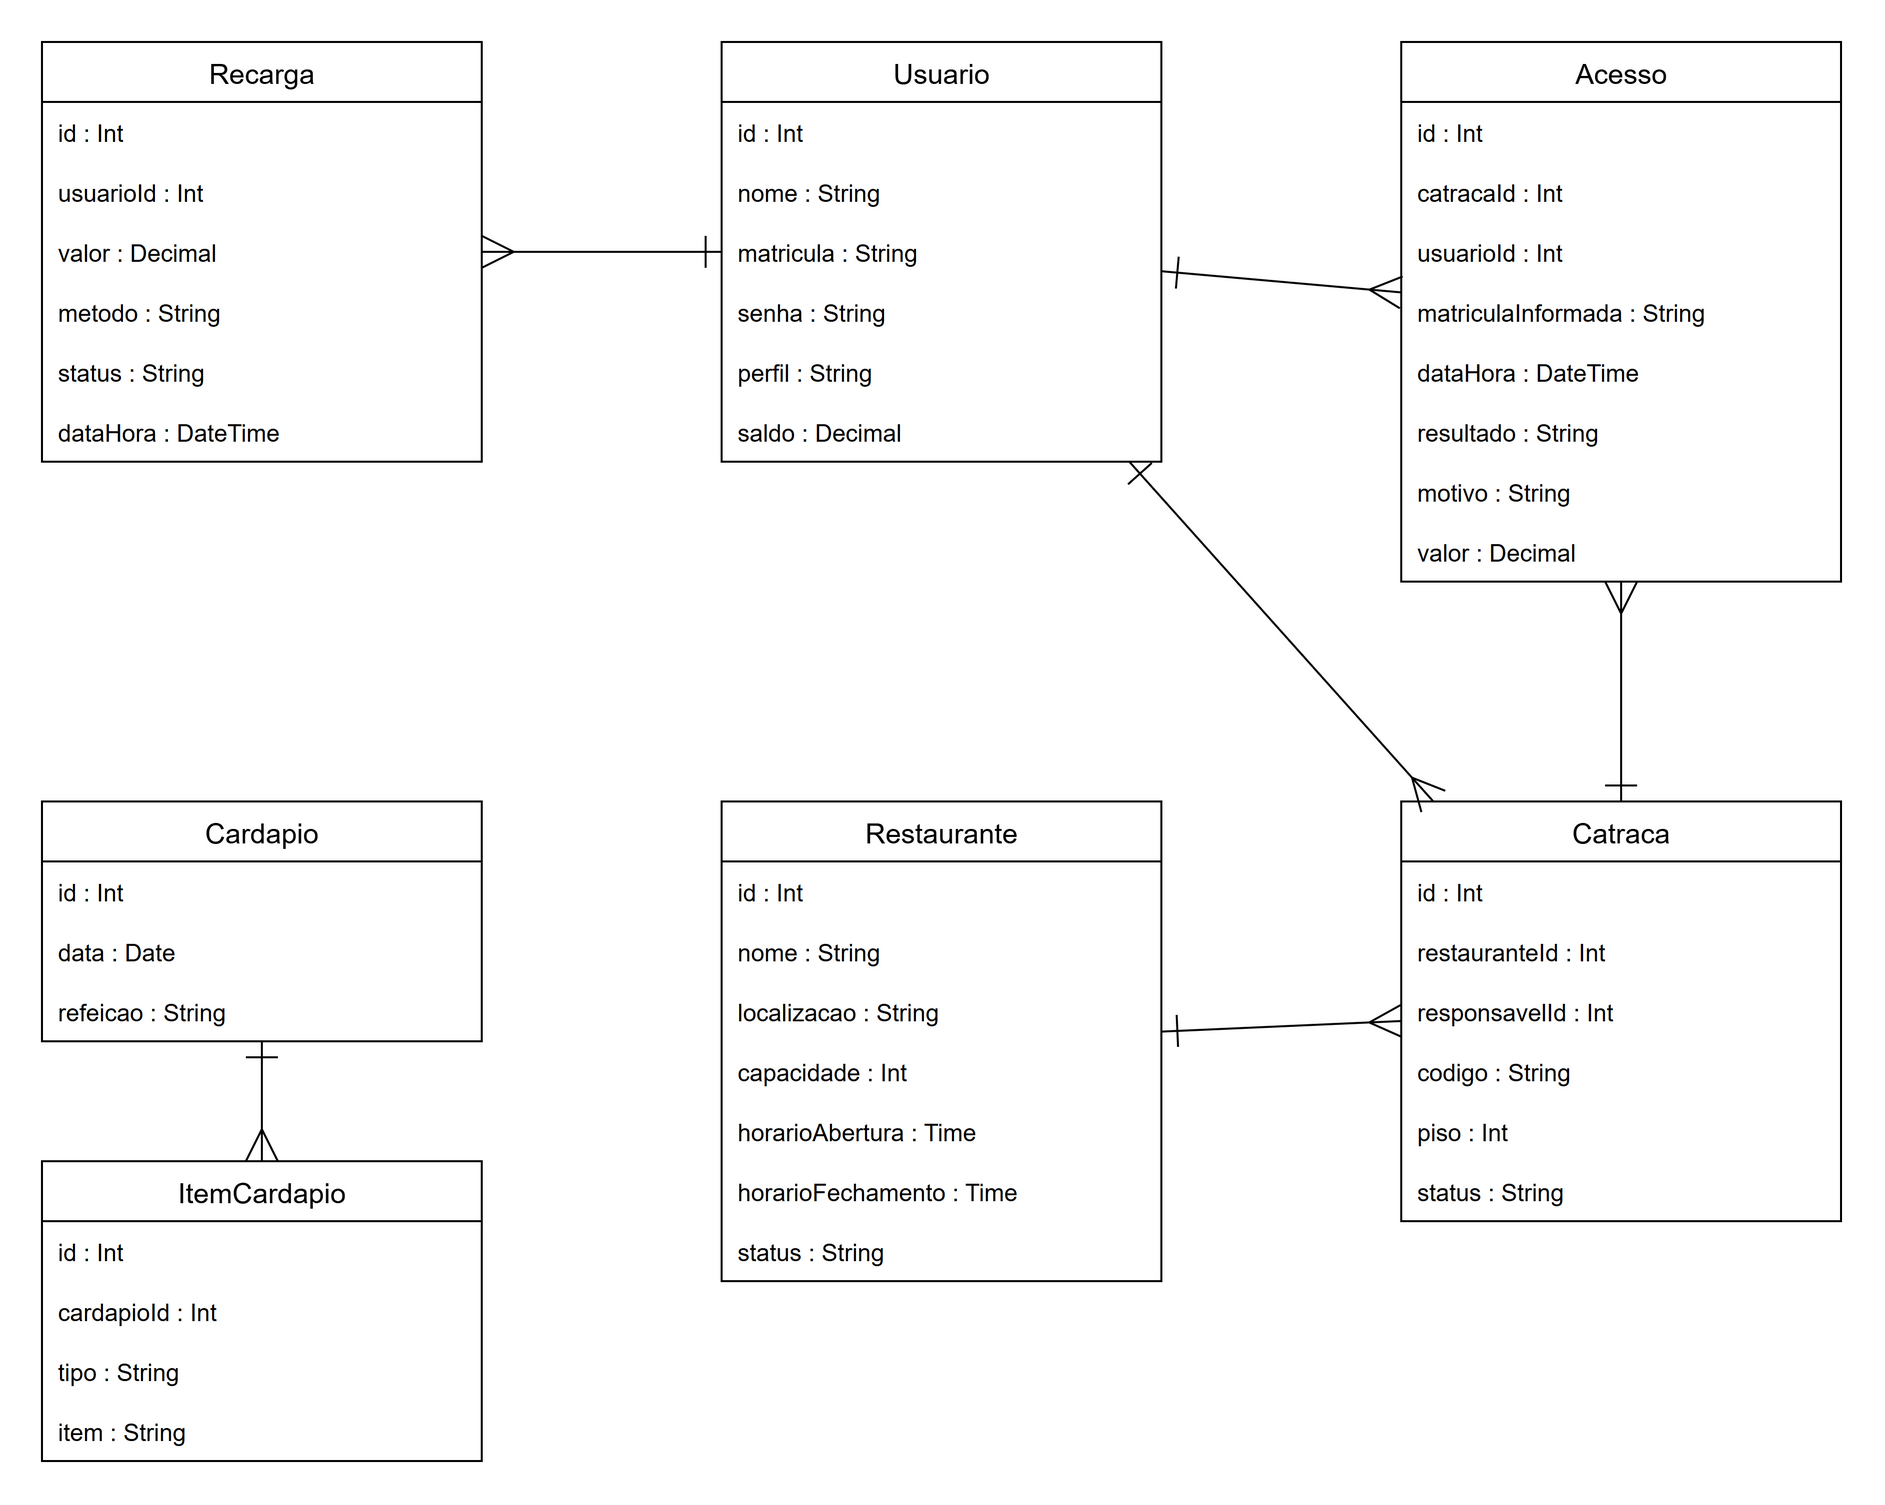
\includegraphics[width=0.9\textwidth]{MER_UnB_RU.png}

    \caption{Modelo Relacional UML da aplicação UnB RU.}

    \label{fig:uml}

\end{figure}

\section*{Investigação Técnica (Spike)}

O spike analisou as 12 telas do protótipo no Figma, exportadas em PDF e SVG, e definiu como transformá-las em views Rails. As telas se organizam em três áreas, e cada área corresponde a um \textit{layout}: o Portal do Estudante (\texttt{estudante}), a Aplicação de Controle (\texttt{operador}) e a Administração (\texttt{administracao}). As rotas são agrupadas por perfil, cada controller exige o perfil correspondente por meio de um \texttt{before\_action}, e os componentes repetidos, como cartões de resumo, filtros, tabelas, selos de status e botões de exportação, ficam em \textit{partials} compartilhados. Os valores de exemplo do Figma (como R\$ 72,00 ou 4.\allowbreak{}820 acessos) correspondem a agregações (\texttt{sum} e \texttt{count}) sobre os modelos. Cada tela é descrita a seguir, com a issue correspondente.

\subsection*{1. Início e Carteira (Issue \#10)}

\begin{itemize}

    \item \textbf{Elementos}: saudação com nome, matrícula e curso; cartão de saldo (R\$ 18,00, equivalente a 4 refeições, tarifa única de R\$ 4,50); estado dos três turnos do dia (encerrado, atual e próximo); cardápio do almoço com as opções padrão, ovolactovegetariana e vegetariana restrita, cada uma com prato principal, guarnições, salada, sobremesa e bebida; aviso de FastPass ativo; botão \textit{Recarregar Saldo}.

    \item \textbf{Rails}: rota \texttt{GET /}, \texttt{InicioController\#\allowbreak{}show}, view \texttt{inicio/\allowbreak{}show.\allowbreak{}html.\allowbreak{}erb} com os partials \texttt{\_cartao\_saldo}, \texttt{\_turnos} e \texttt{\_opcao\_cardapio}.

    \item \textbf{Dados e regras}: o método \texttt{Cardapio.\allowbreak{}atual} escolhe a refeição pelo horário do servidor e carrega os \texttt{ItemCardapio} agrupados por tipo. Sem cardápio cadastrado, a tela exibe que o cardápio ainda não foi disponibilizado, e fora do horário de serviço informa o próximo turno.

\end{itemize}

\subsection*{2. Recarga de Saldo (Issue \#2)}

\begin{itemize}

    \item \textbf{Elementos}: pacotes de 2, 5, 10 e 20 refeições (R\$ 9,00, R\$ 22,50, R\$ 45,00 e R\$ 90,00), campo para outra quantidade, escolha entre PIX e cartão de crédito, resumo com o novo saldo, chave PIX com o botão \textit{Copiar Código} e botão \textit{Confirmar}.

    \item \textbf{Rails}: rotas \texttt{GET /recarga} e \texttt{POST /recarga}, \texttt{RecargasController\#\allowbreak{}new} e \texttt{\#create}, formulário \texttt{form\_with model: @recarga}. Um controller Stimulus calcula o total (quantidade $\times$ R\$ 4,50) e copia o código PIX.

    \item \textbf{Dados e regras}: valores negativos ou nulos são rejeitados. A recarga por PIX nasce \textit{pendente} e passa a \textit{aprovada} na confirmação, e a por cartão sem limite fica \textit{recusada}, sem alterar o saldo. O crédito do saldo ocorre dentro de uma transação (\texttt{ActiveRecord::\allowbreak{}Base.\allowbreak{}transaction}).

\end{itemize}

\subsection*{3. Extrato de Refeições (Issues \#3 e \#11)}

\begin{itemize}

    \item \textbf{Elementos}: três cartões de resumo (total gasto no mês, refeições realizadas e total recarregado); filtros de período, tipo de refeição, restaurante e forma de acesso, com o link \textit{Limpar Filtros}; tabela de lançamentos com data e hora, refeição ou evento, restaurante e catraca, método de acesso, valor (débitos em vermelho e recargas em verde) e comprovante; paginação com itens por página; botões \textit{Exportar PDF} e \textit{Imprimir}.

    \item \textbf{Rails}: rota \texttt{GET /extrato}, \texttt{ExtratosController\#\allowbreak{}index}, partials \texttt{\_resumo}, \texttt{\_filtros}, \texttt{\_tabela} e \texttt{\_vazio}. A exportação é o mesmo caminho com a extensão \texttt{.pdf}, e a impressão utiliza \texttt{window.\allowbreak{}print()} com CSS \texttt{@media print}.

    \item \textbf{Dados e regras}: os lançamentos reúnem \texttt{current\_user.\allowbreak{}recargas} e \texttt{current\_user.\allowbreak{}acessos} em ordem decrescente de data, convertidos por um objeto de apresentação. As datas seguem dd/\allowbreak{}mm/\allowbreak{}aaaa (\texttt{Date.\allowbreak{}strptime}), e data inicial posterior à final gera erro. Sem resultados, o partial \texttt{\_vazio} exibe a mensagem de lista vazia.

\end{itemize}

\subsection*{4. Autenticação Operacional (Issue \#4)}

\begin{itemize}

    \item \textbf{Elementos}: campo de matrícula SIAPE ou usuário, campo de senha (ambos obrigatórios), identificação da unidade e botão \textit{Entrar no Sistema}.

    \item \textbf{Rails}: rotas \texttt{GET /operador/\allowbreak{}entrar} e \texttt{POST /operador/\allowbreak{}entrar}, \texttt{Operador::\allowbreak{}SessoesController\#\allowbreak{}new}, \texttt{\#create} e \texttt{\#destroy}. A tela utiliza o layout \texttt{operador} sem a barra de navegação, que só aparece após o login.

    \item \textbf{Dados e regras}: o modelo \texttt{Usuario} utiliza \texttt{has\_secure\_password}, e o \texttt{create} grava o identificador na sessão. Credenciais incorretas ou não cadastradas exibem ``Credenciais inválidas'', e campos vazios exibem o alerta de preenchimento obrigatório, sempre mantendo a tela de autenticação.

\end{itemize}

\subsection*{5. Configuração de Ponto (Issue \#5)}

\begin{itemize}

    \item \textbf{Elementos}: seleção da unidade operacional, seleção da catraca física agrupada por piso com seu estado (online ou pronta), relógio do servidor sincronizado por NTP, sessão de refeição atual, trava anti-reentrada de 120 minutos, resumo da vinculação e botão \textit{Confirmar e Iniciar Operação}.

    \item \textbf{Rails}: rotas \texttt{GET /operador/\allowbreak{}ponto} e \texttt{PATCH /operador/\allowbreak{}ponto}, \texttt{Operador::\allowbreak{}PontosAcessoController\#\allowbreak{}show} e \texttt{\#update}, partial \texttt{\_catraca\_opcao} e agrupamento com \texttt{group\_by(\&:piso)}. O relógio é atualizado por um controller Stimulus a partir da hora enviada pelo servidor.

    \item \textbf{Dados e regras}: a lista contém apenas restaurantes ativos e catracas ativas do restaurante escolhido. Os identificadores escolhidos ficam na sessão. Confirmar sem selecionar exibe ``Selecione um restaurante para continuar'', e restaurante inativo exibe ``Restaurante indisponível para operação''. Estudantes recebem acesso negado.

\end{itemize}

\subsection*{6. Terminal de Validação (Issue \#6)}

\begin{itemize}

    \item \textbf{Elementos}: horário oficial, alternância entre Modo Comum e Modo Exclusivo FastPass, leitura de QR Code, painel de resultado (acesso liberado ou bloqueado), identificação do estudante, débito e saldo restante, simulador de leituras (\textit{Simular OK}, \textit{Fora Janela} e \textit{Sem Saldo}) e tabela das últimas validações com horário, matrícula, modalidade, valor e status.

    \item \textbf{Rails}: rotas \texttt{GET /operador/\allowbreak{}terminal} e \texttt{POST /operador/\allowbreak{}validacoes}, \texttt{Operador::\allowbreak{}TerminalController\#\allowbreak{}show} e \texttt{Operador::\allowbreak{}ValidacoesController\#\allowbreak{}create}. A resposta do \texttt{create} é um \textit{Turbo Stream} que atualiza o painel de resultado e a tabela sem recarregar a página.

    \item \textbf{Dados e regras}: um objeto de serviço (\texttt{ValidacaoEntrada}) aplica as regras: matrícula com 9 dígitos, estudante cadastrado, catraca disponível e saldo de pelo menos R\$ 4,50. Cada tentativa grava um \texttt{Acesso} liberado ou negado, com o motivo, e a liberação debita o saldo. O simulador fica restrito ao ambiente de desenvolvimento.

\end{itemize}

\subsection*{7. Histórico Local de Acessos (Issue \#7)}

\begin{itemize}

    \item \textbf{Elementos}: título com a catraca, unidade, posto e turno; cartões do turno (giros confirmados, validações FastPass e total debitado); filtros de status e modo; botões \textit{Atualizar Lista} e \textit{Exportar Relatório (CSV/PDF)}; tabela com horário, matrícula, modo de validação, tarifa e status da catraca (liberado, ou bloqueado com o motivo), com as linhas bloqueadas destacadas; paginação.

    \item \textbf{Rails}: rota \texttt{GET /operador/\allowbreak{}historico}, \texttt{Operador::\allowbreak{}HistoricoController\#\allowbreak{}index}, partials \texttt{\_resumo\_turno}, \texttt{\_filtros}, \texttt{\_tabela} e \texttt{\_selo\_status}. A exportação utiliza \texttt{respond\_to} com os formatos \texttt{csv} e \texttt{pdf}.

    \item \textbf{Dados e regras}: a consulta é \texttt{Acesso.\allowbreak{}where(catraca: current\_user.\allowbreak{}catracas)}, restrita às catracas do funcionário, e os filtros atuam sobre \texttt{resultado} e sobre o modo. Funcionário sem catraca vinculada vê a mensagem para procurar o administrador. Os cenários pedem também filtro por período (dd/\allowbreak{}mm/\allowbreak{}aaaa) e hora (HH:MM), ausente da tela.

\end{itemize}

\subsection*{8. Gestão de Restaurantes e Catracas (Issue \#8)}

\begin{itemize}

    \item \textbf{Elementos}: cartões de totais (restaurantes, catracas e corredor FastPass); botões \textit{Cadastrar Restaurante} e \textit{Associar Nova Catraca}; lista de unidades com capacidade total em refeições por hora, catracas ativas e os botões \textit{Editar Unidade} e \textit{Ver Catracas}; catracas agrupadas por piso, com status.

    \item \textbf{Rails}: \texttt{Admin::\allowbreak{}RestaurantesController} (\texttt{index}, \texttt{new}, \texttt{create}, \texttt{edit} e \texttt{update}) e \texttt{Admin::\allowbreak{}CatracasController} (\texttt{create} e \texttt{update}), formulários \texttt{form\_with} e partial \texttt{\_catraca\_card}. A rota de \texttt{destroy} da catraca não existe, e a inativação é uma atualização de status.

    \item \textbf{Dados e regras}: nome único, localização obrigatória, capacidade de 1 a 5000, abertura anterior ao fechamento e código da catraca único dentro do restaurante. Inativar um restaurante inativa as catracas ativas na mesma transação. Restaurante só é removido sem catracas vinculadas, e funcionários acessam a tela apenas para leitura.

\end{itemize}

\subsection*{9. Relatório Global de Operação (Issues \#9 e \#12)}

\begin{itemize}

    \item \textbf{Elementos}: filtros de data contábil, turno e unidade, com o indicador de catracas online; quatro cartões (refeições servidas, arrecadação global, acessos via FastPass e pontualidade); tabela de consolidação por restaurante com acessos, FastPass, pontualidade e arrecadação bruta; métodos de liquidação (PIX e cartão); distribuição por refeição; botões \textit{Exportar CSV} e \textit{Exportar PDF Oficial}.

    \item \textbf{Rails}: rota \texttt{GET /admin/\allowbreak{}relatorio}, \texttt{Admin::\allowbreak{}RelatoriosController\#\allowbreak{}show}, com a classe de consulta \texttt{RelatorioOperacao}, que recebe data, turno e unidade e serve à tela e ao PDF. A exportação utiliza \texttt{respond\_to} e a gem \texttt{prawn}.

    \item \textbf{Dados e regras}: as agregações utilizam \texttt{group(:restaurante\_id)}, \texttt{count} e \texttt{sum(:valor)} sobre \texttt{Acesso}, e \texttt{group(:metodo)} sobre \texttt{Recarga}. O PDF traz o período, a data e hora de emissão e o administrador, só é gerado quando há registros e nunca é enviado pela metade. Apenas o administrador acessa.

\end{itemize}

\subsection*{10. Sorteio FastPass (épico bônus)}

\begin{itemize}

    \item \textbf{Elementos}: passe do próximo turno (contemplado, número do sorteio, validade, turno, janela, catraca, tolerância de 5 minutos, código do passe e botão \textit{Liberar vaga}); ciclo diário de refeições; inscrição no sorteio com escolha da unidade e da janela exclusiva, horário do resultado e botão \textit{Inscrever-se no Sorteio}.

    \item \textbf{Rails}: \texttt{FastpassController\#\allowbreak{}show} e \texttt{InscricoesFastpassController\#\allowbreak{}create} e \texttt{\#destroy}, com os modelos \texttt{InscricaoFastpass} e \texttt{PasseFastpass}. O sorteio é executado por uma tarefa agendada (\texttt{ActiveJob}) 60 minutos antes da abertura do turno.

    \item \textbf{Dados e regras}: cada estudante possui uma inscrição por turno, e a não utilização do passe sem cancelamento gera bloqueio de 24 horas em novos sorteios.

\end{itemize}

\subsection*{11. Turnos e Time-frames (épico bônus)}

\begin{itemize}

    \item \textbf{Elementos}: três turnos (café da manhã, almoço e jantar) com horário, duração, situação e modo FastPass; parâmetros de granularidade (15 minutos), tolerância (3 minutos) e antecedência (2 minutos); grade de lotes ativáveis por clique; opção de pontualidade rígida; botões \textit{Salvar} e \textit{Restaurar Padrão}.

    \item \textbf{Rails}: \texttt{Admin::\allowbreak{}TurnosController\#\allowbreak{}index} e \texttt{\#update}, modelos \texttt{Turno} e \texttt{LoteFastpass}, e um controller Stimulus que alterna o estado de cada lote.

    \item \textbf{Dados e regras}: a tela informa que as alterações chegam às catracas em até 60 segundos, o que corresponde a um cache da configuração com expiração de 60 segundos (\texttt{Rails.\allowbreak{}cache.\allowbreak{}fetch}).

\end{itemize}

\subsection*{12. Vagas e Cotas FastPass (épico bônus)}

\begin{itemize}

    \item \textbf{Elementos}: cartões de cota diária total, taxa de ocupação e capacidade segura por catraca; grade de janelas com a cota, a carga por catraca e um campo de ajuste manual; total ofertado; botões \textit{Redefinir Padrões} e \textit{Aplicar Cotas ao Próximo Sorteio}.

    \item \textbf{Rails}: \texttt{Admin::\allowbreak{}CotasFastpassController\#\allowbreak{}index} e \texttt{\#update}, com atualização em lote por \texttt{fields\_for} e o modelo \texttt{CotaFastpass}.

    \item \textbf{Dados e regras}: a carga por catraca é calculada pela divisão da cota pelo número de catracas ativas, e a cota de uma janela não pode ultrapassar a capacidade segura da catraca.

\end{itemize}

\subsection*{Divergências em relação às features}

\begin{itemize}

    \item A recarga do Figma vende pacotes de refeições, e os cenários tratam de valores em reais.

    \item A autenticação do Figma aceita matrícula SIAPE ou usuário SIGAA/gov.br, e o cenário exige matrícula de 7 dígitos.

    \item O Terminal de Validação do Figma possui os modos Comum e FastPass, ausentes dos cenários de Validação de Entrada.

    \item O histórico local do Figma filtra por status e modo, e os cenários filtram por período e hora.

    \item O Cadastro de Usuário (Issue \#1) não possui tela no Figma, e as telas de FastPass, turnos e cotas não possuem features no repositório.

\end{itemize}

\section*{Considerações Finais}

O modelo reúne as entidades das funcionalidades do grupo e evidencia o vínculo entre restaurantes, catracas e acessos. O spike mostra que as 12 telas do protótipo cabem em três layouts e em um conjunto pequeno de componentes compartilhados. Permanecem a alinhar no grupo as divergências entre as telas do Figma e os cenários.

\end{document}
